%% V:  I have decided to use this template as a template for reports from ZUI
%% for the MDP task. I have planned to create a template just for the course 
%% but then I have decided to just use this template as it is well commented
%% and also quite similar to what I have intended. Occasionally, I have added
%% some comments in the source code - these are marked by 'V:'. I have also removed some parts that seemed unnecessary for the purposes of the course.

%% V: the original template can be found at https://www.sharelatex.com/templates/5851991a93a02abc513710f4.



%% bare_jrnl_compsoc.tex
%% V1.4b
%% 2015/08/26
%% by Michael Shell
%% See:
%% http://www.michaelshell.org/
%% for current contact information.
%%
%% This is a skeleton file demonstrating the use of IEEEtran.cls
%% (requires IEEEtran.cls version 1.8b or later) with an IEEE
%% Computer Society journal paper.
%%
%% Support sites:
%% http://www.michaelshell.org/tex/ieeetran/
%% http://www.ctan.org/pkg/ieeetran
%% and
%% http://www.ieee.org/

%%*************************************************************************
%% Legal Notice:
%% This code is offered as-is without any warranty either expressed or
%% implied; without even the implied warranty of MERCHANTABILITY or
%% FITNESS FOR A PARTICULAR PURPOSE! 
%% User assumes all risk.
%% In no event shall the IEEE or any contributor to this code be liable for
%% any damages or losses, including, but not limited to, incidental,
%% consequential, or any other damages, resulting from the use or misuse
%% of any information contained here.
%%
%% All comments are the opinions of their respective authors and are not
%% necessarily endorsed by the IEEE.
%%
%% This work is distributed under the LaTeX Project Public License (LPPL)
%% ( http://www.latex-project.org/ ) version 1.3, and may be freely used,
%% distributed and modified. A copy of the LPPL, version 1.3, is included
%% in the base LaTeX documentation of all distributions of LaTeX released
%% 2003/12/01 or later.
%% Retain all contribution notices and credits.
%% ** Modified files should be clearly indicated as such, including  **
%% ** renaming them and changing author support contact information. **
%%*************************************************************************


\documentclass[10pt,journal,compsoc,twoside]{IEEEtran}
%
% If IEEEtran.cls has not been installed into the LaTeX system files,
% manually specify the path to it like:
% \documentclass[10pt,journal,compsoc]{../sty/IEEEtran}





% Some very useful LaTeX packages include:
% (uncomment the ones you want to load)





% *** CITATION PACKAGES ***
%
\ifCLASSOPTIONcompsoc
  % IEEE Computer Society needs nocompress option
  % requires cite.sty v4.0 or later (November 2003)
  %\usepackage[nocompress]{cite}
\else
  % normal IEEE
  %\usepackage{cite}
\fi
% cite.sty was written by Donald Arseneau
% V1.6 and later of IEEEtran pre-defines the format of the cite.sty package
% \cite{} output to follow that of the IEEE. Loading the cite package will
% result in citation numbers being automatically sorted and properly
% "compressed/ranged". e.g., [1], [9], [2], [7], [5], [6] without using
% cite.sty will become [1], [2], [5]--[7], [9] using cite.sty. cite.sty's
% \cite will automatically add leading space, if needed. Use cite.sty's
% noadjust option (cite.sty V3.8 and later) if you want to turn this off
% such as if a citation ever needs to be enclosed in parenthesis.
% cite.sty is already installed on most LaTeX systems. Be sure and use
% version 5.0 (2009-03-20) and later if using hyperref.sty.
% The latest version can be obtained at:
% http://www.ctan.org/pkg/cite
% The documentation is contained in the cite.sty file itself.
%
% Note that some packages require special options to format as the Computer
% Society requires. In particular, Computer Society  papers do not use
% compressed citation ranges as is done in typical IEEE papers
% (e.g., [1]-[4]). Instead, they list every citation separately in order
% (e.g., [1], [2], [3], [4]). To get the latter we need to load the cite
% package with the nocompress option which is supported by cite.sty v4.0
% and later. Note also the use of a CLASSOPTION conditional provided by
% IEEEtran.cls V1.7 and later.

% V: I recommend using the biblatex package instead of the package cite.
% You can either load it with default settings:
%\usepackage{biblatex}
% V: or you can set many options manually:
\usepackage[
    style=alphabetic,
    citestyle=authoryear,
    maxbibnames=9,
    maxcitenames=2,
    backend=biber,
    ibidtracker=false,
    ]{biblatex}

% The bibliography is usually in a separate file which is loaded as follows:
% V: The file containing citation descriptions
\bibliography{biblio.bib}



% *** GRAPHICS RELATED PACKAGES ***
%
\ifCLASSINFOpdf
  \usepackage[pdftex]{graphicx}
  % declare the path(s) where your graphic files are
  \graphicspath{{./figures/}}
  % and their extensions so you won't have to specify these with
  % every instance of \includegraphics
  \DeclareGraphicsExtensions{.pdf,.jpeg,.png}
\else
  % or other class option (dvipsone, dvipdf, if not using dvips). graphicx
  % will default to the driver specified in the system graphics.cfg if no
  % driver is specified.
  % \usepackage[dvips]{graphicx}
  % declare the path(s) where your graphic files are
  % \graphicspath{{../eps/}}
  % and their extensions so you won't have to specify these with
  % every instance of \includegraphics
  % \DeclareGraphicsExtensions{.eps}
\fi
% graphicx was written by David Carlisle and Sebastian Rahtz. It is
% required if you want graphics, photos, etc. graphicx.sty is already
% installed on most LaTeX systems. The latest version and documentation
% can be obtained at: 
% http://www.ctan.org/pkg/graphicx
% Another good source of documentation is "Using Imported Graphics in
% LaTeX2e" by Keith Reckdahl which can be found at:
% http://www.ctan.org/pkg/epslatex
%
% latex, and pdflatex in dvi mode, support graphics in encapsulated
% postscript (.eps) format. pdflatex in pdf mode supports graphics
% in .pdf, .jpeg, .png and .mps (metapost) formats. Users should ensure
% that all non-photo figures use a vector format (.eps, .pdf, .mps) and
% not a bitmapped formats (.jpeg, .png). The IEEE frowns on bitmapped formats
% which can result in "jaggedy"/blurry rendering of lines and letters as
% well as large increases in file sizes.
%
% You can find documentation about the pdfTeX application at:
% http://www.tug.org/applications/pdftex






% *** MATH PACKAGES ***
%
% V: this is very useful package. I believe that almost any report you'll
% write will use it.
\usepackage{amsmath}
% A popular package from the American Mathematical Society that provides
% many useful and powerful commands for dealing with mathematics.
%
% Note that the amsmath package sets \interdisplaylinepenalty to 10000
% thus preventing page breaks from occurring within multiline equations. Use:
%\interdisplaylinepenalty=2500
% after loading amsmath to restore such page breaks as IEEEtran.cls normally
% does. amsmath.sty is already installed on most LaTeX systems. The latest
% version and documentation can be obtained at:
% http://www.ctan.org/pkg/amsmath

% V:
\usepackage{amssymb}
\usepackage{amsmath}
\usepackage{amsfonts}
\usepackage{mathtools}


% *** SPECIALIZED LIST PACKAGES ***
%
%\usepackage{algorithmic}
% algorithmic.sty was written by Peter Williams and Rogerio Brito.
% This package provides an algorithmic environment fo describing algorithms.
% You can use the algorithmic environment in-text or within a figure
% environment to provide for a floating algorithm. Do NOT use the algorithm
% floating environment provided by algorithm.sty (by the same authors) or
% algorithm2e.sty (by Christophe Fiorio) as the IEEE does not use dedicated
% algorithm float types and packages that provide these will not provide
% correct IEEE style captions. The latest version and documentation of
% algorithmic.sty can be obtained at:
% http://www.ctan.org/pkg/algorithms
% Also of interest may be the (relatively newer and more customizable)
% algorithmicx.sty package by Szasz Janos:
% http://www.ctan.org/pkg/algorithmicx




% *** ALIGNMENT PACKAGES ***
%
%\usepackage{array}
% Frank Mittelbach's and David Carlisle's array.sty patches and improves
% the standard LaTeX2e array and tabular environments to provide better
% appearance and additional user controls. As the default LaTeX2e table
% generation code is lacking to the point of almost being broken with
% respect to the quality of the end results, all users are strongly
% advised to use an enhanced (at the very least that provided by array.sty)
% set of table tools. array.sty is already installed on most systems. The
% latest version and documentation can be obtained at:
% http://www.ctan.org/pkg/array


% IEEEtran contains the IEEEeqnarray family of commands that can be used to
% generate multiline equations as well as matrices, tables, etc., of high
% quality.




% *** SUBFIGURE PACKAGES ***
%\ifCLASSOPTIONcompsoc
%  \usepackage[caption=false,font=footnotesize,labelfont=sf,textfont=sf]{subfig}
%\else
%  \usepackage[caption=false,font=footnotesize]{subfig}
%\fi
% subfig.sty, written by Steven Douglas Cochran, is the modern replacement
% for subfigure.sty, the latter of which is no longer maintained and is
% incompatible with some LaTeX packages including fixltx2e. However,
% subfig.sty requires and automatically loads Axel Sommerfeldt's caption.sty
% which will override IEEEtran.cls' handling of captions and this will result
% in non-IEEE style figure/table captions. To prevent this problem, be sure
% and invoke subfig.sty's "caption=false" package option (available since
% subfig.sty version 1.3, 2005/06/28) as this is will preserve IEEEtran.cls
% handling of captions.
% Note that the Computer Society format requires a sans serif font rather
% than the serif font used in traditional IEEE formatting and thus the need
% to invoke different subfig.sty package options depending on whether
% compsoc mode has been enabled.
%
% The latest version and documentation of subfig.sty can be obtained at:
% http://www.ctan.org/pkg/subfig




% *** FLOAT PACKAGES ***
%
%\usepackage{fixltx2e}
% fixltx2e, the successor to the earlier fix2col.sty, was written by
% Frank Mittelbach and David Carlisle. This package corrects a few problems
% in the LaTeX2e kernel, the most notable of which is that in current
% LaTeX2e releases, the ordering of single and double column floats is not
% guaranteed to be preserved. Thus, an unpatched LaTeX2e can allow a
% single column figure to be placed prior to an earlier double column
% figure.
% Be aware that LaTeX2e kernels dated 2015 and later have fixltx2e.sty's
% corrections already built into the system in which case a warning will
% be issued if an attempt is made to load fixltx2e.sty as it is no longer
% needed.
% The latest version and documentation can be found at:
% http://www.ctan.org/pkg/fixltx2e


%\usepackage{stfloats}
% stfloats.sty was written by Sigitas Tolusis. This package gives LaTeX2e
% the ability to do double column floats at the bottom of the page as well
% as the top. (e.g., "\begin{figure*}[!b]" is not normally possible in
% LaTeX2e). It also provides a command:
%\fnbelowfloat
% to enable the placement of footnotes below bottom floats (the standard
% LaTeX2e kernel puts them above bottom floats). This is an invasive package
% which rewrites many portions of the LaTeX2e float routines. It may not work
% with other packages that modify the LaTeX2e float routines. The latest
% version and documentation can be obtained at:
% http://www.ctan.org/pkg/stfloats
% Do not use the stfloats baselinefloat ability as the IEEE does not allow
% \baselineskip to stretch. Authors submitting work to the IEEE should note
% that the IEEE rarely uses double column equations and that authors should try
% to avoid such use. Do not be tempted to use the cuted.sty or midfloat.sty
% packages (also by Sigitas Tolusis) as the IEEE does not format its papers in
% such ways.
% Do not attempt to use stfloats with fixltx2e as they are incompatible.
% Instead, use Morten Hogholm'a dblfloatfix which combines the features
% of both fixltx2e and stfloats:
%
% \usepackage{dblfloatfix}
% The latest version can be found at:
% http://www.ctan.org/pkg/dblfloatfix




%\ifCLASSOPTIONcaptionsoff
%  \usepackage[nomarkers]{endfloat}
% \let\MYoriglatexcaption\caption
% \renewcommand{\caption}[2][\relax]{\MYoriglatexcaption[#2]{#2}}
%\fi
% endfloat.sty was written by James Darrell McCauley, Jeff Goldberg and 
% Axel Sommerfeldt. This package may be useful when used in conjunction with 
% IEEEtran.cls'  captionsoff option. Some IEEE journals/societies require that
% submissions have lists of figures/tables at the end of the paper and that
% figures/tables without any captions are placed on a page by themselves at
% the end of the document. If needed, the draftcls IEEEtran class option or
% \CLASSINPUTbaselinestretch interface can be used to increase the line
% spacing as well. Be sure and use the nomarkers option of endfloat to
% prevent endfloat from "marking" where the figures would have been placed
% in the text. The two hack lines of code above are a slight modification of
% that suggested by in the endfloat docs (section 8.4.1) to ensure that
% the full captions always appear in the list of figures/tables - even if
% the user used the short optional argument of \caption[]{}.
% IEEE papers do not typically make use of \caption[]'s optional argument,
% so this should not be an issue. A similar trick can be used to disable
% captions of packages such as subfig.sty that lack options to turn off
% the subcaptions:
% For subfig.sty:
% \let\MYorigsubfloat\subfloat
% \renewcommand{\subfloat}[2][\relax]{\MYorigsubfloat[]{#2}}
% However, the above trick will not work if both optional arguments of
% the \subfloat command are used. Furthermore, there needs to be a
% description of each subfigure *somewhere* and endfloat does not add
% subfigure captions to its list of figures. Thus, the best approach is to
% avoid the use of subfigure captions (many IEEE journals avoid them anyway)
% and instead reference/explain all the subfigures within the main caption.
% The latest version of endfloat.sty and its documentation can obtained at:
% http://www.ctan.org/pkg/endfloat
%
% The IEEEtran \ifCLASSOPTIONcaptionsoff conditional can also be used
% later in the document, say, to conditionally put the References on a 
% page by themselves.




% *** PDF, URL AND HYPERLINK PACKAGES ***
%
%\usepackage{url}
% url.sty was written by Donald Arseneau. It provides better support for
% handling and breaking URLs. url.sty is already installed on most LaTeX
% systems. The latest version and documentation can be obtained at:
% http://www.ctan.org/pkg/url
% Basically, \url{my_url_here}.



% V:  *** PACKAGES I FREQUENTLY USE ***

% V: for (not only) czech characters
\usepackage[utf8]{inputenc}

% V: for english language
\usepackage{csquotes}
\usepackage[english]{babel}

% V: fonts
\usepackage[T1]{fontenc}


% V: for coloured text - for notes in the draft
\usepackage{color}

% V: allows for creation fictional files inside a single tex file
% \usepackage{filecontents}

% V: plotting using just the LaTeX
% this results in nice vectorized plots but might take a little bit time to compile thus if you have a lot of plots you might need to install LaTeX locally instead of using ShareLatex or Overleaf as those might time out. 
% \usepackage{pgfplots}
% \usepackage{tikz}

% V: for nice ordinals
\usepackage{nth}

% V: for links
\usepackage{hyperref}
\hypersetup{
     colorlinks   = true,
     citecolor    = blue,
     filecolor=cyan,      
     urlcolor=magenta,
}

% V: for references
% this allows for use \cref{} instead of \ref which take care of automatically
% naming the referenced object, i.e. instead of writing '... in fig.
% \ref{fig:mylilfigure}' you write ' ... in \cref{fig:mylilfigure}'
\usepackage{cleveref}


% V: for listing code
\usepackage{listings}
\definecolor{codegreen}{rgb}{0,0.4,0}
\lstset{
    frameround=fttt,
    language=python,
    numbers=left,
    breaklines=true,
    keywordstyle=\color{blue}\bfseries, 
    basicstyle=\ttfamily\color{black},
    numberstyle=\color{black},
    stringstyle=\color{codegreen},
    }
\lstdefinelanguage{none}{
  identifierstyle=
}

% V: for including matlab code
%\usepackage[numbered,framed]{matlab-prettifier}

% V: for subfigures
%\usepackage{caption}
%\usepackage{subcaption}

% V: for matrices
%\usepackage{bm}

% correct bad hyphenation here
\hyphenation{op-tical net-works semi-conduc-tor}

% V: just to make writing matrices and vectors easy
\newcommand{\matr}[1]{\mathbf{#1}} % undergraduate algebra version
%\newcommand{\matr}[1]{#1}          % pure math version
%\newcommand{\matr}[1]{\bm{#1}}     % ISO complying version

\renewcommand{\vec}[1]{\mathbf{#1}} %if bold vectors wanted


% V: declaring some useful math operators
\DeclareMathOperator*{\argmin}{arg\,min}
\DeclareMathOperator*{\argmax}{arg\,max}




\begin{document}



%
% paper title
% Titles are generally capitalized except for words such as a, an, and, as,
% at, but, by, for, in, nor, of, on, or, the, to and up, which are usually
% not capitalized unless they are the first or last word of the title.
% Linebreaks \\ can be used within to get better formatting as desired.
% Do not put math or special symbols in the title.
\title{Assignment 5 \\ GridWorld}

\author{B4B36ZUI, BE4B36ZUI}



% The paper headers
\markboth{LS2018, Assignment 5 --- GridWorld}%
{B4B36ZUI, BE4B36ZUI}
% The only time the second header will appear is for the odd numbered pages
% after the title page when using the twoside option.
% 



% for Computer Society papers, we must declare the abstract and index terms
% PRIOR to the title within the \IEEEtitleabstractindextext IEEEtran
% command as these need to go into the title area created by \maketitle.
% As a general rule, do not put math, special symbols or citations
% in the abstract or keywords.
\IEEEtitleabstractindextext{%
\begin{abstract}
The assignment 5 focuses on Markov decision processes (MDPs) used for solving a GridWorld examples and is worth 12 points in total. The GridWorld consists of a rectangular grid of cells and the goal is to navigate an agent to reach the highest reward using non--deterministic actions. The assignment is to be implemented in Python 3.6 using provided codes. The assignment consists of both implementation part and experimental part.
\end{abstract}
}


% make the title area
\maketitle




\section{Introduction}\label{sec:introduction}





% The very first letter is a 2 line initial drop letter followed
% by the rest of the first word in caps (small caps for compsoc).
% 
% form to use if the first word consists of a single letter:
% \IEEEPARstart{A}{demo} file is ....
% 
% form to use if you need the single drop letter followed by
% normal text (unknown if ever used by the IEEE):
% \IEEEPARstart{A}{}demo file is ....
% 
% Some journals put the first two words in caps:
% \IEEEPARstart{T}{his demo} file is ....
% 
% Here we have the typical use of a "T" for an initial drop letter
% and "HIS" in caps to complete the first word.
\IEEEPARstart{T}{he} goal of this assignment is to find optimal decision policy of an agent maximizing its reward in a GridWorld MDP problem (see \href{http://cw.fel.cvut.cz/wiki/_media/courses/b4b36zui/mdps_show.pdf}{slides} or \href{https://en.wikipedia.org/wiki/Markov_decision_process}{Wikipedia} for details). A GridWorld consists of a rectangular grid of $m \times n$ cells. The cells are described using coordinate system with $[0,0]$ in top left corner. An agent can make for different actions --- it can go one cell north, east, south, and west from the cell it is occupying. The actions are not deterministic and intended action will be executed only with probability $p$ (\text{action\_proba}) and some other action will be executed with probability $1-p$. More specifically, only the action that are neighbouring the intended cardinal direction might be executed instead and each of them with uniform probability, i.e. if the agent's intended action is \textit{north}, it will be executed with probability $p$ and action \textit{east} or \textit{west} will be executed instead with probability $\frac{1-p}{2}$. Each action has an associated cost $c$ (\texttt{action\_cost}), which, for the purposes of this assignment, is identical for each action. This cost is applied only when the cell where the action would have ended has no associated reward --- if the cell $[i,j]$ has an associated reward $r_{i,j}$, the reward overrides the cost. (Note, if you wanted to apply the action cost $c$ in any case, just change \texttt{=} at line 536 to \texttt{+=}).

In all the predefined worlds, the cells with defined reward are also set be terminal states where the agent ends when he reaches them. It is recommend for your experiments to keep the set of reward states the same as the set of the terminal state. A reward (or a cost if it is negative) is obtained if the associated cell is reached by the agent.

\section{Algorithms}\label{sec:algoritgms}
While the MDPs can be solved by both linear programming and dynamic programming, this task focuses on the latter --- namely, only two variants of dynamic programming for solving the MDP are needed: \textit{value iteration} and \textit{policy iteration}. The dynamic programming approach consists of iterative estimation of the values of individual states $V(s)$ and choosing the best policy $\pi(s)$ for deciding for action $a$ from the set of actions $\mathbb{A}$ for each state 0 $s$ from the set of states $\mathbb{S}$.

First, the action are evaluated using known valuation of states $V_{n-1}(s)$ and the transitional probabilities $P(s' | a, s)$ where $s'$ is the target state, $s$ is the current state, and $a$ is the executed action:

\begin{equation}
    Q_{n}(s,a) = \sum_{s' \in \mathbb{S}} P(s' | a, s)\left(R(s') + \gamma V_{n-1}(s')\right)
\end{equation}

where $R(s')$ is the reward for reaching state $s'$ and $\gamma \in [0,1]$ is the discount factor.

The optimal policy $\pi_{n}(s)$ is chosen as
\begin{equation}
    \pi_{n}(s) = \argmax_{\substack{
        a \in \mathbb{A}
        }
    } Q_{n}(s,a)
\end{equation}

and finally, the valuation of states $V_n$ is recomputed:

\begin{equation}
    V_n = \sum_{s' \in \mathbb{S}} P(s' | \pi_n(s), s)\left(R(s') + \gamma V_{n-1}(s')\right)
\end{equation}

\subsection{Value iteration}
The \textit{value iteration} algorithm skips explicitly computing the optimal policy and consists of a single step repeated until convergence criterion is met:
\begin{equation}
    V_n = \max_{a \in \mathbb{A}} \left( \sum_{s' \in \mathbb{S}} P(s' | a, s)\left(R(s') + \gamma V_{n-1}(s')\right)\right)
\end{equation}

\subsection{Policy iteration}
The \textit{policy iteration} consists of two steps --- computation the optimal policy $\pi_n(s)$ and evaluation of states $V_n(s)$ given the policy $\pi_n(s)$. The evaluation of states for given policy might be either computed solving set of equations or iteratively similarly as in the \textit{value iteration}. The assignment uses the iterative version which consists of repeated computation of $Q_{n}(s,a)$ and $V_n$ until the $V_n$ meets the convergence criterion.

\section{Implementation}
There are several implementation details that are worth. First, while, the functions are defined as multidimensional arrays --- $R(s)$ is replaced by an array $\matr{R}$ of shape $|\mathbb{S}|$ where $\matr{R}[s] = R(s)$, $P(s' | a, s)$ is replaced by $\matr{P}$ of shape $|\mathbb{S}| \times |\mathbb{A}| \times |\mathbb{S}|$ where $\matr{P}[s,a,s'] = P(s' | a, s)$. Also $V_n(s)$ is saved as an array $\matr{V}_n$ of shape $|\mathbb{S}|$  and $Q_n(s,a)$ as $\matr{Q}_n$ of shape $|\mathbb{S}| \times |\mathbb{A}|$.

The set of states $\mathbb{S}$ consists of all cells from the grid and a \textbf{terminal sink state} which is an added state that cannot be left (all action with lead back to it with probability 1) and which has no reward for reaching it. All action from the states \textbf{on} the grid that are considered to be terminal leads to the sink state to prevent repeated application of rewards that are associated with such states.

\subsection{Environment}
The task is to be implemented and the provided codes are in \textbf{python 3.6}. The other necessary packages are \textit{NumPy} \cite{numpy}, \textit{matplotlib} \cite{matplotlib}, \textit{seaborn} \cite{seaborn}.

It is recommended to use \href{https://www.anaconda.com/download/}{Anaconda distribution} which also contains a package manager which allows to install many pre-compiled packages (which is especially beneficial when using Windows as it is often problematic to compile packages there).

\section{Task}
The task consists of two parts, an implementative one and experimental one. The goal of the implementative part is to implement missing parts of several functions while the experimental parts consists of several small experiments with the GridWorld. The output of the assignment are the implemented codes, script (or Jupyter notebook) for launching the experiments, and report.

\subsection{Implementative part [4p]}
Your goal is to implement several helper functions (\lstinline{Q_from_V}, \lstinline{Q2V}, \lstinline{Q2Vbypolicy}, and \lstinline{Q2policy}), evaluation of the MDP for given policy (\lstinline{evaluate_policy}), value iteration (\lstinline{value_iteration}), and policy iteration (\lstinline{policy_iteration}) in the file \texttt{ZUI\_MDP.py}. You are also provided a set of test cases (\texttt{test\_ZUI\_MDP.py}) that can be used for testing your implementation using e.g. \texttt{unittest} or \texttt{nosetests} modules. It is not necessary to use the tests but it is recommended as the correctness of your implementation will be tested similarly (mostly same tests with just different parameterization). 

\subsection{Experimental part [6p]}
Once you have correctly implemented all the necessary functions, your goal is to experiment with the GridWorld MDPs. You are required to do at least 4 different experiments from which two are assigned (and are the same for all of you) and you are required to come up with your own ideas for the other two. All the experiments have to be thoroughly described in the report --- the settings, used GridWorld parametrization, goals of the experiments, results (including visualization) and (if necessary) a conclusion. 

\subsubsection{Experiment 1: Policy switching based on action probability}
Your goal is to analyze how the optimal policy changes with the changes of action probability $p$ for the predefined GridWorld \texttt{3x4}. The output is to be a list of values of $p$ for which there occurs a change in the optimal policy and also a plot showing the valuation of states 0, 3, 6, 8, 9, 10, and 11 together with thresholds where the policy change occurs. The plot should be similar to plot \cref{fig:experiment_1_3x3} which shows the Experiment 1 for the GridWorld \texttt{3x3} and states 0, 1, 3, 6, and 8. The probability $p$ should be on the x axis and the valuation on the y axis.

\begin{figure}[t]
    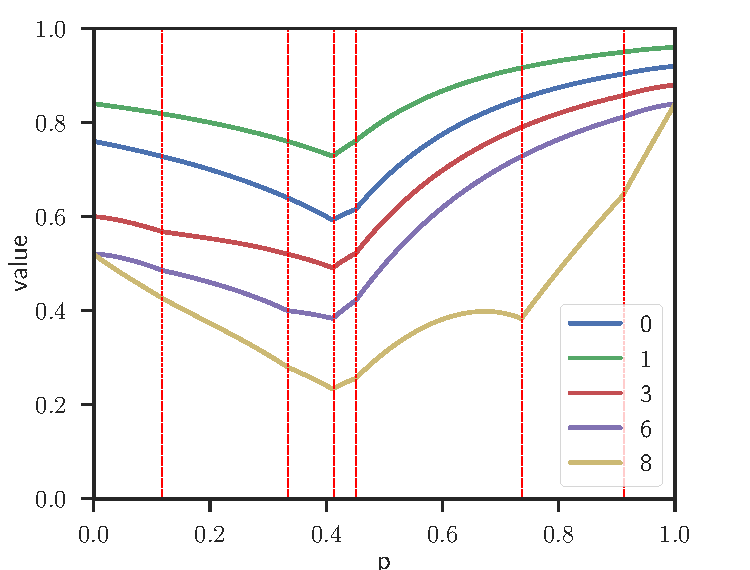
\includegraphics[width=8cm]{figures/experiment_1_3x3.pdf}
    \centering
    \caption{Example of output of Experiment 1 for the GridWorld \texttt{3x3} and states 0, 1, 3, 6, and 8}
    \label{fig:experiment_1_3x3}
\end{figure}


\subsubsection{Experiment 2: Policy switching based on action cost}
Your goal is to analyze how the optimal policy changes with the changes of action costs $c \in [0,\infty]$ for the predefined GridWorld \texttt{5x5}. The output is to be a list of values of $c$ for which there occurs a change in the optimal policy. You also should show plots of the several most interesting policies (you can use method \lstinline{GridWorld.plot}) --- the exact policies you show are up to you.

\subsubsection{Experiments 3 and 4 (or more)}
You are required to come up with your own experiments that should be at least as complex as the previous two experiments. The possibilities are almost endless, e.g. measuring the runtime based on the size of the grid, influence of both action cost $c$ and action probability $p$ on certain states (you would plot a heatmap where on the $x$ axis would be action probability $p$, on the $y$ axis would be action cost $c$ and the color would encode the value of the given state),or simple evolutionary algorithms for finding good policies (using function \lstinline{evaluate_policy} for evaluation the objective or writing a custom evaluation function that solves equations for evaluation the policy instead of iterating). \textbf{At least one} of the experiments \textbf{should be different} from the experiments described above (i.e. it is not sufficient to just take the experiments described above and just change the GridWorld instance to another predefined GridWorld instance).

You are required to include stand-alone scripts named \texttt{<username>\_experiment\_<n>.py} (e.g. \texttt{kuncvlad\_experiment\_2.py}) that are launchable in the described environment. For experiments running longer than 5 minutes, write the approximate running time in the report. Your experiment can be also in \href{http://jupyter.org/}{Jupyter notebooks} (\texttt{.ipynb}).


\subsection{Report [2p]}
You are required to describe all the steps in a short report. The report has no fixed length limit but it is evaluated on the basis of completeness and correctness of presented information. You can get up to \textbf{2 points} for the neatness and formal requirements of the report --- e.g. your figures should have captions summarizing what is there, you should reference figures from the text (usage of \texttt{\\cref\{\}} is recommended), your report should have logical structure, etc. You are required to hand in the report in the PDF format (any PDF format that graders can open is acceptable but it is guaranteed that format \texttt{PDF/A} is fine). You are \textbf{not required} to use \LaTeX{}  but it is \textbf{highly recommended}, furthermore a \LaTeX{} template \texttt{ZUI\_template.tex} is provided for your use (and it is also \textbf{recommended} to use the template).

\section{Grading}
The whole assignment is worth \textbf{12 points in total}. The implementative part is for \textbf{4 points in total} --- implementation of the helper functions is worth \textbf{1 point} and the implementation of \lstinline{evaluate_policy}, \lstinline{value_iteration}, and \lstinline{policy_iteration} is worth \textbf{1 point for each function}. The experimental part is worth \textbf{6 points in total} where each experiment is worth \textbf{1.5 point} (Note that the points are transferable between experiments --- a great experiment might offset poorer experiment). The final \textbf{2 points} are for the report itself. Summary of the grading is in \cref{tab:grading}.


\begin{table}[h]
\centering
 \begin{tabular}{l c} 
    subtask & points \\ 
    \hline
    helper functions & 1 \\
    {\lstinline|evaluate_policy|} & 1\\
    {\lstinline|value_iteration|} & 1 \\
    {\lstinline|policy_iteration|} & 1 \\
    \hline
    Experiment 1 & 1.5 \\ 
    Experiment 2 & 1.5 \\ 
    Experiment 3 & 1.5 \\ 
    Experiment 4 & 1.5 \\ 
    \hline
    report & 2 \\ \hline \hline
    \textbf{total} & \textbf{12}\\
    \hline
 \end{tabular}
 \caption{Summary of points receivable for the assignment.}
 \label{tab:grading}
\end{table}

\section{Deadline}
The deadline for submission into the \href{https://cw.felk.cvut.cz/brute/student/}{upload system} is 22.5.2018 23:59:59 CES.
\printbibliography




% if have a single appendix:
%\appendix[Proof of the Zonklar Equations]
% or
%\appendix  % for no appendix heading
% do not use \section anymore after \appendix, only \section*
% is possibly needed

% use appendices with more than one appendix
% then use \section to start each appendix
% you must declare a \section before using any
% \subsection or using \label (\appendices by itself
% starts a section numbered zero.)
%


\appendices
\section{Notes}
Please follow the \href{http://cw.fel.cvut.cz/wiki/courses/b4b36zui/tasks/task4-gridworld-en}{course webpage} and the \href{https://cw.felk.cvut.cz/forum/forum-1494-page-1.html}{forum} for updates and additional information. In case of any questions, please write to the forum or write an email to \texttt{kuncvlad@fel.cvut.cz}.
\subsection{\LaTeX{} editor}
Unless you have installed \LaTeX{} locally, it is recommended to either use \href{https://www.sharelatex.com?r=8e97ffd0&rm=d&rs=b}{ShareLaTeX} or \href{https://www.overleaf.com/signup?ref=54db136ac70d}{Overleaf} --- these sites provide online editors and also have many predefined templates and also allow online collaboration (which might be useful for your other projects). Both of them provide almost the same functionality (they actually merged into one a year ago but they still provide both services separately).

If you have \LaTeX{} installed \textbf{locally}, it is recommended to set the \texttt{matplotlib} with \LaTeX{} which allows using \LaTeX{} code inside the figure --- e.g. for the legend or axis labels.

\subsection{Using Unittests}
While the tests can be launched from terminal, you can launch them also directly from the \href{https://www.jetbrains.com/pycharm/}{PyCharm IDE}. The usage is very simple and is shown in \cref{fig:nosetests,fig:nosetests_results}.

\begin{figure}[t]
    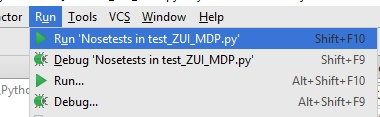
\includegraphics[width=8cm]{figures/pycharm_nosetests.jpg}
    \centering
    \caption{You can run the tests similarly as any other script --- just keep active the test file and click on \texttt{Run}}
    \label{fig:nosetests}
\end{figure}


\begin{figure}[t]
    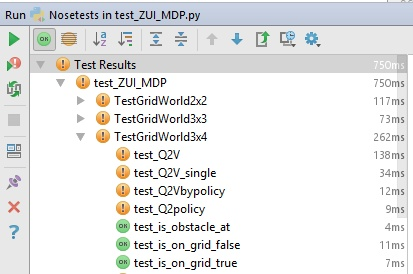
\includegraphics[width=8cm]{figures/pycharm_nosetests_results.jpg}
    \centering
    \caption{The results of the test shows in the lower left corner by default. You can click on any of the tests to see details (and the script output in case you print anything).}
    \label{fig:nosetests_results}
\end{figure}


\subsection{Virtual environment}
It is recommended to use separate virtual environment for your assignment. If you are using the Anaconda distribution, you can create new environment using

\begin{lstlisting}[language=none]
conda create -n ZUI_MDP python=3.6 numpy seaborn matplotlib
\end{lstlisting}

which can be then activated using \lstinline[language=none]{activate ZUI_MDP} on Windows and \lstinline[language=none]{source activate ZUI_MDP} on Linux. More details are available in the \href{https://conda.io/docs/user-guide/tasks/manage-environments.html}{documentation}.

\subsection{Saving figures}
You should save the figures in a vectorized format which is better for publication. This can be done easily in python using 

\begin{lstlisting}[language=python]
plt.savefig('your_filename.pdf', dpi=500, transparent=True)
\end{lstlisting}

% that's all folks
\end{document}


